\documentclass[11pt]{beamer}
\usetheme{Pittsburgh}
\usepackage[utf8]{inputenc}
\usepackage[english]{babel}
\usepackage{amsmath}
\usepackage{amsfonts}
\usepackage{amssymb}
\usepackage{mathrsfs} 
\usefonttheme[onlymath]{serif}

\defbeamertemplate*{title page}{customized}[1][]
{
  \usebeamercolor[fg]{titlegraphic}\inserttitlegraphic
  \flushleft
  \medskip
  \usebeamerfont{title}\inserttitle\par
  \medskip
  \usebeamerfont{subtitle}\usebeamercolor[fg]{subtitle}\insertsubtitle\par
  \vfill
  \usebeamerfont{author}\insertauthor\par
  \usebeamerfont{institute}\insertinstitute\par
  \medskip
  \usebeamerfont{date}\insertdate\par

}
\newenvironment{proenv}{\only{\setbeamercolor{local structure}{fg=green}}}{}
\newenvironment{conenv}{\only{\setbeamercolor{local structure}{fg=red}}}{}

\setbeamertemplate{footline}[text line]{%
  \parbox{\linewidth}{\vspace*{-8pt}MSI SS14\hfill\insertshortauthor\hfill\insertframenumber}}
\setbeamertemplate{navigation symbols}{}

\titlegraphic{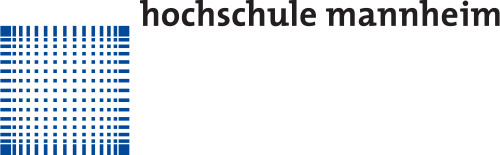
\includegraphics[scale=0.25]{logo.png}}
\author{Horst Schneider, Patrick Beedgen}
\title{Understanding Eventual Consistency}
\subtitle{MSI Presentation SS2014}
\institute{Hochschule Mannheim} 
\date{June 17th, 2014} 
\begin{document}

\begin{frame}
\titlepage
\end{frame}

\begin{frame}
\frametitle{Introduction}
\begin{quotation}
\glqq ...the 
storage system guarantees that if no 
new updates are made to the object, 
eventually all accesses will return the 
last updated valuee\grqq
\linebreak
--W. Vogels (2009)
\end{quotation}
\end{frame}



\begin{frame}
\frametitle{Introduction}
\framesubtitle{Interpretations of Eventual Consistency}
\begin{footnotesize}

Interpretation 1:

\begin{quotation}
"When you read data[...], the response might not reflect the results of a recently completed write operation. The response might include some stale data. Consistency across all copies of the data is usually reached within a second; so if you repeat your read request after a short time, the response returns the latest data."
\end{quotation}

Interpretation 2:

\begin{quotation}
"This sort of system we term “single writer eventual consistency”.  So what are its properties?\linebreak (1) A client could read stale data. (2) The client could see out-of-order write operations. [...] So this is our weakest form of consistency - eventually consistent with out of order reads in the short term."
\end{quotation}
\end{footnotesize}
\end{frame}

\begin{frame}

\frametitle{Introduction}
\framesubtitle{Interpretations of Eventual Consistency}
\begin{footnotesize}
DynamoDB Documentation
\begin{quotation}
"When you read data[...], the response might not reflect the results of a recently completed write operation. The response might include \textbf{some stale data}. Consistency across all copies of the data is \textbf{usually reached within a second}; so if you repeat your read request after a short time, the response returns the latest data."
\end{quotation}

MongoDB Documentation
\begin{quotation}
"This sort of system we term “single writer eventual consistency”. So what are its properties?\linebreak (1)A client could read stale data. \linebreak(2)The client could see out-of-order write operations.[...]\linebreak So this is our weakest form of consistency - eventually consistent with \textbf{out of order reads} in the short term."
\end{quotation}
\end{footnotesize}
\end{frame}

\begin{frame}
\frametitle{The Problem}
\begin{itemize}
\item Disparate and low-level formalisms\linebreak 
\textit{consistency model is tied to system implementation}
\item Weak guarantees\linebreak 
\textit{in realistic scenarios updates \textbf{never} stop}
\item Conflict resolution policies\linebreak 
\textit{resolution of conflicts in multiple replicas}
\item Combinations of different consistency levels\linebreak 
\textit{strong consistency may be needed at certain times} 
\end{itemize}
\begin{large}
\ensuremath{\Rightarrow}
\end{large}
Some sort of formalism is needed to define semantics of Eventual Consistency
\end{frame}

\begin{frame}
\frametitle{Agenda}
\tableofcontents
\end{frame}

\section{Replicated Data Types}

\begin{frame}
\frametitle{Replicated Data Types}
\begin{itemize}
\item A replicated database stores \textbf{objects} \(\mathrm{Obj} = \{x,y,\dots\} \)
\pause
\item Every object \(x \in \mathrm{Obj}\) has
\begin{itemize}
\item a \textbf{value} \(\in \mathrm{Val}\)
\item a \textbf{type} type\((x) \leftrightarrow \tau \)
\item \textbf{operations} \(\mathrm{Op}_{\mathrm{type}(x)}\) that a client can perform on it
\pause
\end{itemize}
\item Two examples: Int Register \textbf{intreg}, Counter \textbf{ctr}
\end{itemize}

\begin{align*}
\mathrm{Op}_\mathrm{ctr} &= \mathrm{\{rd, inc\}} \\
\mathrm{Op}_\mathrm{intreg} &= \mathrm{\{rd, wr(}k \mathrm{)|} k \in \mathbb{Z} \mathrm{\}}
\end{align*}
\end{frame}

\begin{frame}
\frametitle{Replicated Data Types}
\framesubtitle{Sequential Data Type Specification}
In a \textit{strongly consistent system}, the semantics of a data type can be specified by a function \\
\begin{equation*}
S_{\tau}\ : \mathrm{Op}_\tau^+ \rightarrow \mathrm{Val}
\end{equation*}
\pause
Example:
\begin{align*}
S_{\mathrm{ctr}} \mathrm{(\sigma rd)} &= \mathrm{(number\ of\ inc\ operations\ in\ \sigma);} \\
\onslide<3->{S_{\mathrm{intreg}} \mathrm{(\sigma rd)} &= k;\ \mathrm{if\ wr(0) \sigma = \sigma_1 wr(}k\mathrm{) \sigma_2\ and} \\
 & \mathrm{\sigma_2 \ does\ not\ contain\ wr\ operations} \\}
\onslide<4->{
S_{\mathrm{intreg}} \mathrm{(\sigma\ wr(}k\mathrm{))} &= S_{\mathrm{ctr}} \mathrm{(\sigma\ inc)} = \bot; }
\end{align*}
(e.g. \(\sigma =\{ \mathrm{rd\ rd\ wr(5)\ wr(6)\ rd\} }\) or \(\sigma =\{ \mathrm{rd\ rd\ inc\ inc\ rd\} } \) )

\end{frame}

\begin{frame}
\frametitle{Replicated Data Types}
\framesubtitle{Semantics of Eventual Consistency}
\begin{itemize}
\item semantics of eventually consistent systems are harder to formalize
\item concurrent operations on the same object happen on multiple replicas
\item each replica executes operations immediately, updating other replicas later
\item different implementation strategies for replicated data types
\end{itemize}
\end{frame}

\begin{frame}
\frametitle{Replicated Data Types}
\framesubtitle{Conflict Resolution Strategies}
\begin{columns}
\begin{column}{5cm}
\begin{figure}
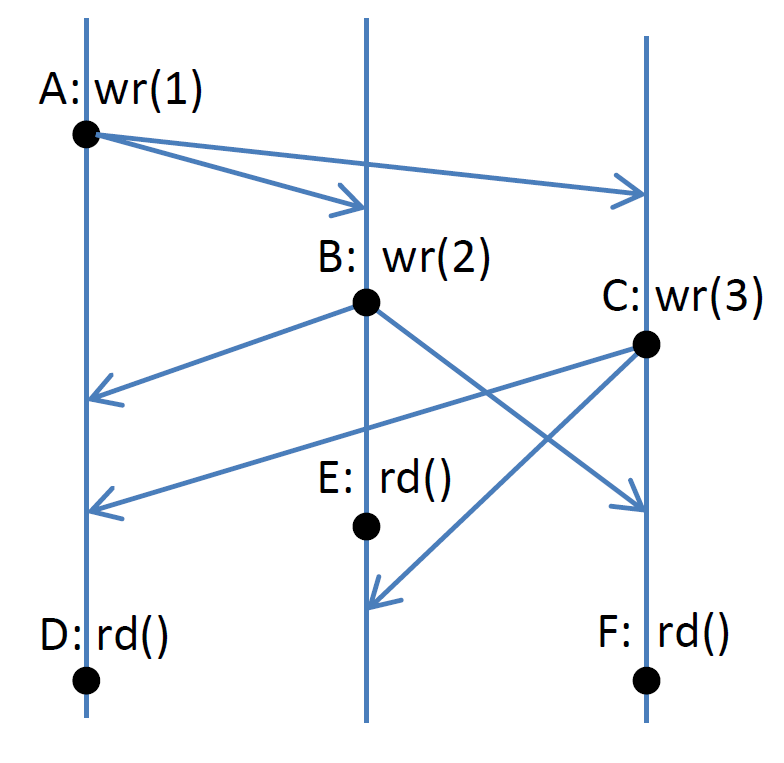
\includegraphics[scale=0.3]{update_replicas_highres.png}
\end{figure}
\end{column}
\begin{column}{5cm}
\pause
\begin{enumerate}
\item Make concurrent operations commutative
\pause
\item Order concurrent operations
\pause
\item Flag conflicts (let the user decide)
\pause
\item Resolve conflicts semantically
\end{enumerate}
\end{column}
\end{columns}
\end{frame}

\begin{frame}
\frametitle{Replicated Data Types}
\framesubtitle{Replicated Data Type Specification}
\begin{itemize}
\item \(S_{\tau}\) is not strong enough to formalize these strategies
\pause
\item visibility and order of preceding operations have to be included
\pause
\item \(F_\tau\): takes an \textbf{operation context} and returns a \textbf{value}
\end{itemize}

\begin{center}
\(F_\tau(C) \in \mathrm{Val}\) \\
\end{center}
\pause
\begin{itemize}
\item operation context \(C\) adds \textbf{visibility} and \textbf{arbitration relations} to preceding operations:
\end{itemize}

\begin{center}
\(C = (f, V, \mathrm{ar}, \mathrm{vis})\) \\
\pause
\(u \xrightarrow{\mathrm{vis}} v, \mathrm{vis} \subseteq V \times V  \) \\
\pause
\(u \xrightarrow{\mathrm{ar}} v, \mathrm{ar} \subseteq V \times V  \)
\end{center}

\end{frame}


\begin{frame}
\frametitle{Replicated Data Types}
\framesubtitle{Replicated Data Type Specification}
Example: Strategy \textbf{Make Concurrent Calls Commutative}
\begin{align*}
F_{\mathrm{ctr}} \mathrm{(inc}, V, \mathrm{vis, ar)} &= \bot; \\
F_{\mathrm{ctr}} \mathrm{(rd}, V, \mathrm{vis, ar)} &= \mathrm{(the\ number\ of\ inc\ operations\ in\ } V);
\end{align*}
\pause
Example: Strategy \textbf{Order Concurrent Operations}
\begin{align*}
F_{\mathrm{intreg}} \mathrm{(inc}, V, \mathrm{vis, ar)} &= S_{\mathrm{intreg}}(V^{\mathrm{ar}} f) \\
\end{align*}
\end{frame}

\section{Axiomatic Specification Framework}

\begin{frame}
\frametitle{Axiomatic Specification Framework}
\framesubtitle{Session and Action}
\begin{itemize}
\item clients wish to perform operations in a common context
\item \textbf{sessions} provide a way to track client identity for operations
\item an \textbf{action} is a tuple \((e,s,[x.f:k])\)
\begin{itemize}
\item \(e\): unique identifier
\item \(s\): session id \(\in \mathrm{SId}\)
\item \([x.f:k]\): object, operation and return value
\end{itemize}
\end{itemize}
\pause
Example:

\begin{center}
\(a = (1af3c, 17, [x.rd: k]);\ \mathrm{type(}x\mathrm{)} = \mathrm{intreg}\)
\end{center}
\end{frame}

\begin{frame}
\frametitle{Axiomatic Specification Framework}
\framesubtitle{History and Execution}
\begin{itemize}
\item the set of all actions that happen in a database is denoted as \(\mathrm{Act}\)
\item a \textbf{history} \((A,\mathrm{so})\) is a set of actions \(A \subseteq \mathrm{Act}\) and a \textbf{session order} relation \(\mathrm{so} \subseteq A \times A \)
\item an \textbf{execution} \(X = (A, \mathrm{so, vis, ar})\) enhances the history with visibility and arbitration relations
\item we can now extract an operation context for any action in any session, providing a deterministic return value
\end{itemize}

\end{frame}

\begin{frame}
\frametitle{Axiomatic Specification Framework}
\framesubtitle{Levels of Eventual Consistency}
\begin{itemize}
\item With these replicated data types we can define multiple forms of eventual consistency
\begin{itemize}
\item Basic eventual consistency
\item Ordering guarantees
\item On-demand consistency strengthening
\end{itemize}
\item Every form contains multiple axioms
\end{itemize}
\end{frame}

\begin{frame}
\frametitle{Axiomatic Specification Framework}
\framesubtitle{Basic Eventual Consistency Axioms}
\begin{itemize}
\item Axioms a database implementation has to apply to offer basic eventual consistency
\item Well-Formedness Axioms
\begin{itemize}
\item SOwf, ARwf, VISwf
\end{itemize}
\item Data Type Axiom
\begin{itemize}
\item RVAL
\end{itemize}
\item Basic Eventual Consistency axioms
\begin{itemize}
\item EVENTUAL
\item THINAIR
\end{itemize}

\end{itemize}
\end{frame}

\begin{frame}
\frametitle{Axiomatic Specification Framework}
\framesubtitle{Session guarantees}
\begin{itemize}
\item Axioms that ensure that databases stay consistent within a single session with a client
\item !RYW!, MR, WYRV, WFRA, MWV, MWA
\end{itemize}
\end{frame}

\begin{frame}
\frametitle{Axiomatic Specification Framework}
\framesubtitle{Causal Consistency Axioms}
\begin{itemize}
\item POCV, POCA, COCV, COCA
\end{itemize}
\end{frame}

\begin{frame}
\frametitle{Conclusion}
\begin{itemize}
\item<pro@1-> the paper provides a way to \textbf{precisely specify eventually consistent systems} in a common notation
\item<pro@1-> \textbf{every aspect of a system is covered}, from data types to client interaction
\item<pro@1-> specifications are \textbf{independent of implementation details}
\item<con@1-> still \textbf{very theoretical}, no tools available to map between specifications and implementation 
\item<con@1-> the framework is \textbf{not suitable for programmers}, as it is very abstract and not easily understandable and applicable
\end{itemize}
\end{frame}

\begin{frame}
\begin{center}
\begin{Huge}
Discussion
\end{Huge}
\end{center}
\end{frame}

\end{document}
